\chapter{Les Missions réalisées}
\section{Enjeux et cadre des missions effectuées}
Ma première mission était la réalisation d'une application mobile multi-plateforme 
reprennant les fonctionnalités du site web client tout en prenant en compte 
les différences d'expérience utilisateur qu'apporte une interface tactile.\newline

Les outils et technologies utilisées pour cette mission sont les suivantes:

\begin{figure}[!h]
    \centering
    \begin{minipage}[b]{0.4\textwidth}
      
\includegraphics[width=\textwidth]{Images/ionic-logo}
    \end{minipage}
    \hfill
    \begin{minipage}[b]{0.4\textwidth}
      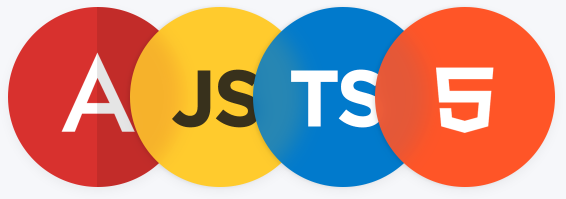
\includegraphics[width=\textwidth]{Images/ajsthtml5}
    \end{minipage}
  \end{figure}

\begin{itemize}
    \item Ionic + cordova
    \item Git comme outils de versionning de code source
    \item Npm comme gestionnaire de librairie 
    \item Visual Studio Code
    \item GitLab pour l'hebergement du code source et la gestion de projet \newline
\end{itemize} 

Mon choix c'est porté sur Ionic pour la rapidité avec laquelle on peut développer une application 
et ce sur les platformes iOS et Android sans avoir à faire du code natif spécifiques 
aux plateforme de plus j'avais déja des compétence en technologie web.

La seconde mission était la refonte totale du site web client qui contient aussi l'API pour 
l'application mobile, ce nouveau site nommé web3 doit avoir les mêmes fonctionnalitées que 
la version précédente tout en utilisant la puissance des nouvelles technologies. \newline

\begin{itemize}
    \item client-side: version Progressive Web App de l'application mobile 
    \item server-side: Asp.net Core 
    \item persistance: base de donnée NexusDB
    \item Git comme outils de versionning de code source 
    \item GitLab pour l'hebergement du code source et la gestion de projet 
    \item Visual Studio Code \newline
\end{itemize}



\section{Présentation d'une mission à fort enjeux: le site client}
Le site web client est la facade directement visible de nos clients c'est donc un produit crucial pour
l'entreprise, il m'a été confié la création du nouveau site web, appelé en interne web3 car il s'agit de la troisième
refonte du site.

j'ai eu totale liberté pour le choix des technologies utilisés, le web2 est basé sur un stack vieillissant: asp.net webforms et jquery.
De plus, la qualité du code et sa maintenabilité est extrèmement faible rendant difficile et ce de manière 
exponentielle, l'ajout de fonctionnalitées et la correction de bugs. 

Pour les choix techniques j'ai choisis de rester sur l'utilisation du langage C\# pour deux raisons, tout d'abord 
je maitrise ce langage depuis de nombreuses années et ensuite c'est le langage utilisé dans la réalisation de tout les 
autres logiciels au sein de l'entreprise ce qui assure une certaine homogeneité et enfin cela me permet 
aussi de reprendre le code de l'ancien site client plus facilement. \newline

L'architecture du web2 était completement incorrecte, utilisant le C\# comme langage purement procédural plutot que 
comme langage objet, aucune des bonnes pratiques ne sont respecté ce qui rend le code hautement dupliqué 
et difficile à maintenir, de plus aucun test unitaires n'etait mis en place rendant difficile la non-regressions.

La première étape fut d'analyser ce qui appartenait purement à la partie métier et d'isoler les composants 
techniques relatif à l'application et à la persistance des données: \newline

\begin{figure}[h]
	\centering
	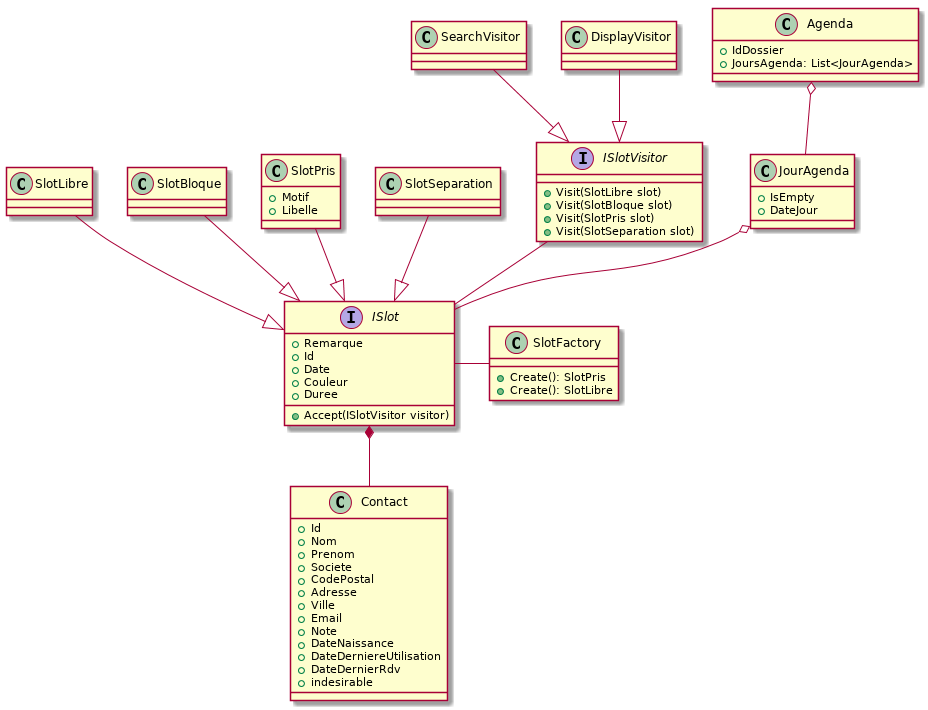
\includegraphics[width=1\linewidth]{Images/slotmodelold}
	\caption{classes métier pour l'agenda}
	\label{fig:domainagenda}
\end{figure}

Cette partie ne concerne que les classes métier de l'agenda, chaque agenda est composé de jour 
qui sont eux-mêmes composés de créneaux (slot) qui peuvent avoir plusieurs états, tout les 
états ne peuvent pas être representé de la même manière car ils correspondent plutôt à 
des sous état tel que le fait qu'un rdv pris soit un rdv web pris via le site web Doctolib 
ou de l'un de nos autres partenaires. 
J'ai du trouver et isoler les propriété et différent états des slot par moi pour avoir une 
architecture correcte, non présente sur le web2.  \newline \newpage

Avec ces classes réalisées je me suis penché sur l'implémentation du reste de l'architecture, 
j'ai opté pour une architecture hexagonale, la partie métier serait un noyau central avec 
lequel le reste de l'application interargirait, cela permettrait ainsi de 
verifier les règles métier avec des test unitaires et d'isoler ces classes avec le reste 
de l'application permettant par ailleurs de porter ce noyau rapidement dans 
d'autres application futures. \newline

\begin{figure}[!h]
    \centering
    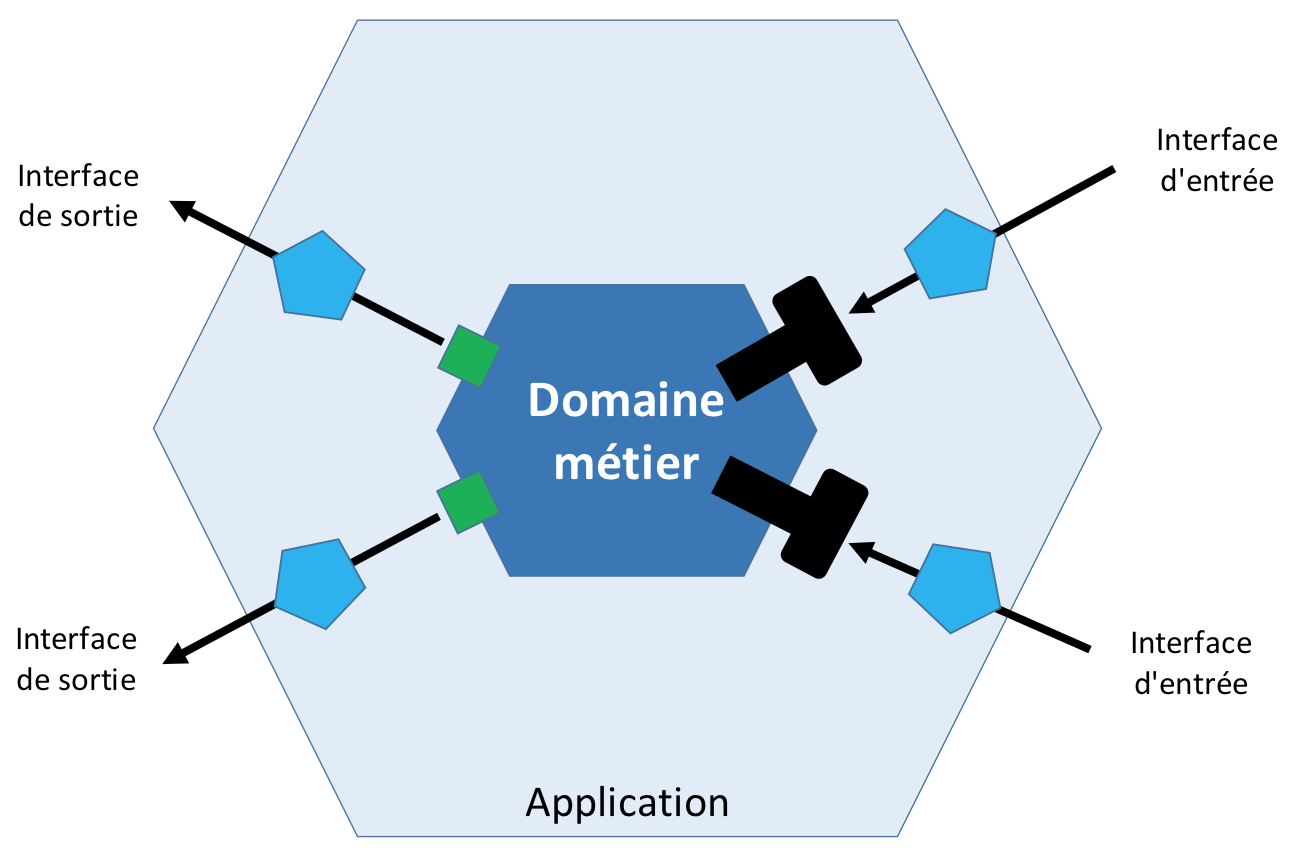
\includegraphics[width=0.6\linewidth]{Images/hexarch}
    \caption{Architecture Hexagonale}
    \label{fig:archhexa}
\end{figure}

Avec une architecture hexagonale, les classes métier communique vers l'exterieur via des "port" et 
des "adapter", les ports sont en fait des interface qui definissent des rôles à remplir 
et les adapter sont les implémentation de ces interfaces, les adapter "remplissent un contrat".

\begin{figure}[h]
	\centering
	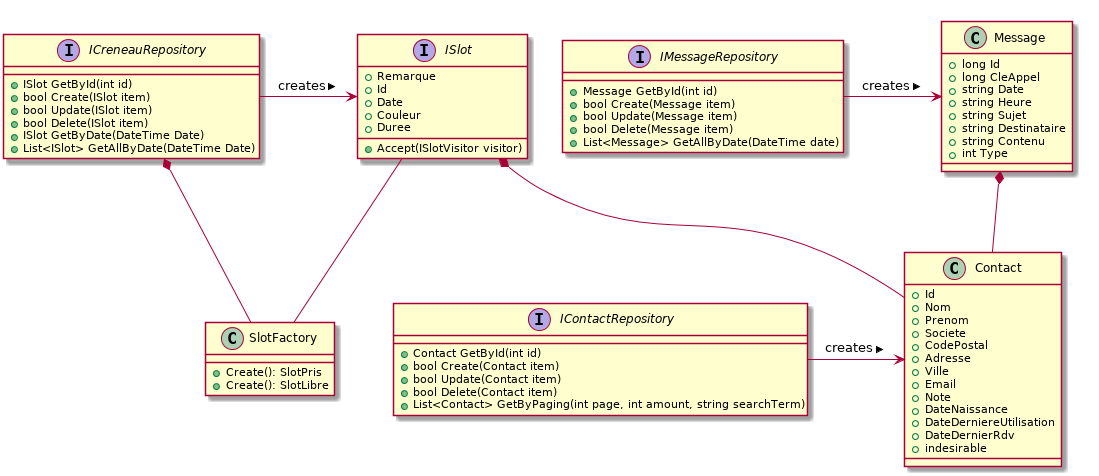
\includegraphics[width=1\linewidth]{Images/slotumlpart1}
	\caption{ exemple d'implémentation des repository }
	\label{fig:otherrepo}
\end{figure}

Les Repository sont l'implémentation d'un interface d'entrée, ils permettent l'interaction de façon 
abstraite avec un support de persistance tel qu'une base de données, le noyau métier ne connais pas 
les dessous technique, cela facilite les test unitaires puisque l'on peu alors utiliser 
des adapteurs qui retournent des données fixe pour les tests. Dans le cas du web3 la grande 
partie des interface d'entrée vont être de l'accès aux données tandis que pour les interfaces
de sortie cela peut être les controller d'ASP.net core ou les requêtes http envoyées 
par l'application mobile. \newline


j'ai ensuite entièrement séparé le noyau métier dans une librairie à part referencé dans 
le projet principal pour plus de clareté et pour permettre l'evolution indépendante du site 
et du noyau qui ont chacun leur depot git, le code client-side est dans le depo du site 
mais j'ai pour objectif de rendre ce code commun entre l'application mobile et le site web.

\section{Bilan et recul sur les missions}
Pour les deux missions j'ai eu totale liberté dans mes choix qui fut à la fois un avantage mais 
aussi une preuve du manque de gestion de projet au sein de l'entreprise, je n'avais 
aucun cahier des charges et les règles métiers n'etaient pas clairement définies,
j'ai du donc établir par moi même le cahier des charge et lister les nouvelles fonctionnalitées 
en me basant sur l'ancien site web et son code qui n'a d'ailleurs pas facilité la tache. \newline

pour l'application j'ai du aussi me baser sur le website et m'auto-former aux bonnes pratiques 
à appliquer à l'expérience utilisateur et l'interface graphique puisqu'une application
n'a pas du tout les mêmes contraintes qu'un site web. \newline

En prenant du recul je me suis rendu que le choix du framework Ionic pour l'application mobile
était un choix judicieux mais seulement à court terme, il est en effet assez difficile de maintenir toute 
application basé sur le javascript et l'environement node car les outils et la qualité 
d'un environement de déveleppement basé sur ces techno est assez médiocre, les librairie 
deviennent incompatibles ou non d'une version sur l'autre, il est assez difficile 
de débugger certaines erreurs à cause de l'epaisseur conséquente du stack de technologies
utilisées. Si je n'avais pas eu d'aussi forte contraintes de temp pour produire un résultat 
j'aurais utilisé le framework Xamarin qui aurait encore plus augmenté la portabilité 
du code puisque j'aurais pu utiliser le noyau métier du web3 dans l'application
ce qui aurait permis de réduire le temp de développement et peut être arriver 
à produire un résultat aussi rapidement qu'avec l'utilisation du framework Ionic, 
au moment des choix technologique j'ai peut être donc fait preuve d'un manque de vision génerale
et sur le long terme. \newline


